\documentclass[a4paper,12pt]{article}

\usepackage[a4paper,margin=1.7cm]{geometry}
\usepackage[english]{babel}
\usepackage[utf8]{inputenc}
\usepackage{amsmath}
\usepackage{graphicx}
\usepackage{subcaption}
\usepackage{siunitx}
\setcounter{MaxMatrixCols}{20}

\newcommand{\hinf}{\mathcal{H}_\infty}
\newcommand{\Hinf}{\(\hinf\)}

\title{Implementation of Mass{\'e} et al.'s \Hinf\ Controller}
\author{J{\'e}r{\'e}mie~X.~J.~Bannwarth}
\date{30 November 2018}

\begin{document}
    \maketitle

    \section{Introduction}

        This document describes the implementation of the controller presented by Mass{\'e} et al.~\cite{MasseEtAl2018} on the quadcopter model introduced in our AIAA Journal paper~\cite{BannwarthEtAl2018}. The main goal behind this task is to gain a better understanding of the \Hinf\ controller design process.
        
        In their paper, Mass{\'e} et al.\ present a simulation model for a standard quadcopter frame, making use of the propeller aerodynamic model developed by Khan and Nahon~\cite{KhanNahon2013,KhanNahon2015}. They subsequently describe and evaluate the performance of two linear station keeping controllers; a LQR controller and a \Hinf\ controller.

        Initially, an attempt at replicating the multirotor model used by Mass{\'e} et al.\ was made. Replicating the model would enable to ensure the controller has been implemented properly by comparing results with those presented in the paper. In addition, the propeller model could be reused in the `Aerodynamic Modelling' section of the thesis as a point of comparison. However, several issues listed in Section~\ref{sec:issues} arose. As a consequence, it was decided to instead implement the \Hinf\ controller on the model presented in our AIAA Journal paper~\cite{BannwarthEtAl2018}, which will be described in the first part of this report.

    \section{Structure of the Controller}

        The controller block diagram is shown in Figure~\ref{fig:ctrl_block_diag}.
        
        \begin{figure}[h!]
            \centering%
            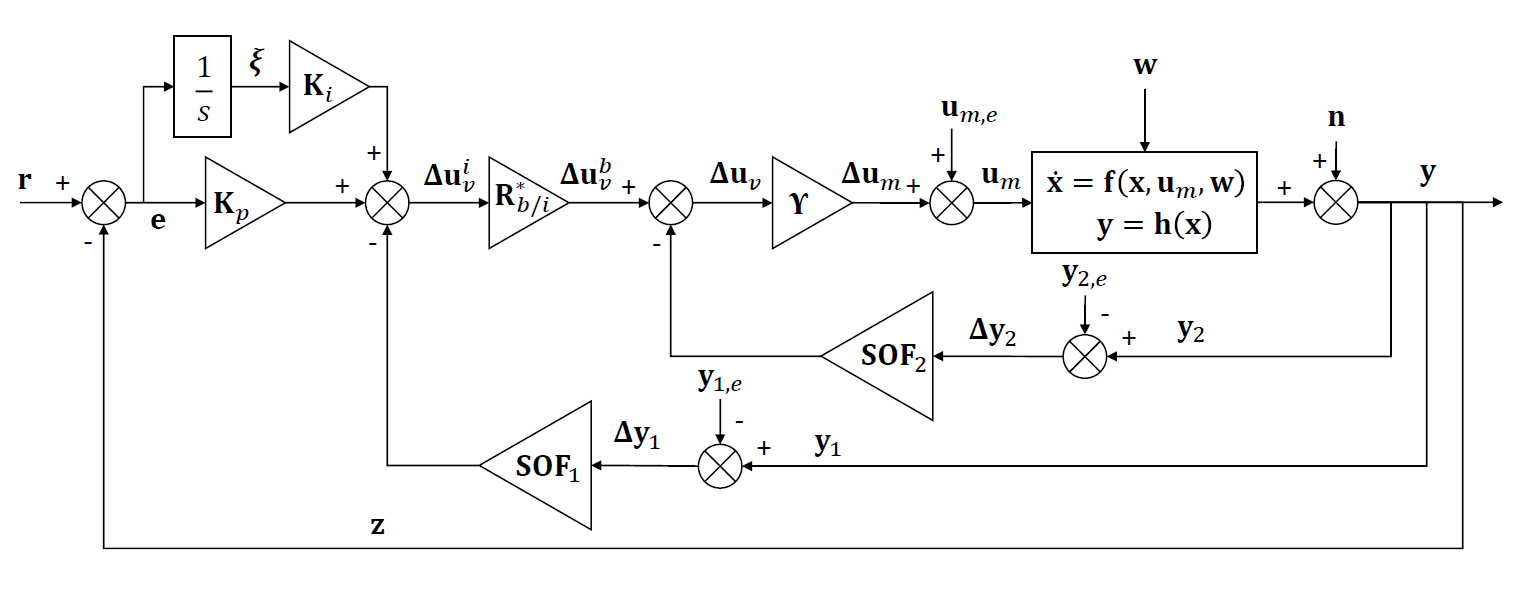
\includegraphics[width=16cm]{ctrl_block_diag.png}%
            \caption{Block diagram of Mass{\'e} et al.'s \Hinf\ controller.}\label{fig:ctrl_block_diag}
        \end{figure}

        The state vector is defined as
        \begin{equation}
            \mathbf{x} = \begin{bmatrix}
                {\mathbf{x}_q}^\top & {\mathbf{x}_m}^\top
            \end{bmatrix}^\top
        \end{equation}
        where \(\mathbf{x}_q\) represents the states of the motors and \(\mathbf{x}_q\) represents the rest of the states of the UAV:
        %
        \begin{equation}
            \mathbf{x}_q = \begin{bmatrix} u & v & w & p & q & r & x & y & z & \phi & \theta & \psi \end{bmatrix}^\top .
        \end{equation}
        %
        where \(u\), \(v\), and \(w\) are the linear velocities of the UAV in the body frame, and \(p\), \(q\), \(r\) are the angular velocities of the UAV in the body frame. The remaining states are the standard pose of the UAV in the world frame.

        The input vector is \(\mathbf{u}_m = \begin{bmatrix} u_1 & u_2 & u_3 & u_4 \end{bmatrix}^\top\), where \(u_j\) represents the control signal sent to motor \(j\), where motor 1 is located to the front left, motor 2 to the back left, etc. It is obtained by multiplying the virtual control input \(\mathbf{u}_v = \begin{bmatrix} F_{z,d} & M_{x,d} & M_{y,d}  & M_{z,d} \end{bmatrix}^\top\) by the mixing matrix \(\mathbf{\Upsilon}\). As our current simulation model still uses the north-west-up convention, the mixing matrix is different from that presented in the original paper and is defined as
        %
        \begin{equation}
            \mathbf{\Upsilon} = \frac{1}{4}
            \begin{bmatrix}
                1 &  1 & -1 &  1 \\
                1 &  1 &  1 & -1 \\
                1 & -1 &  1 &  1 \\
                1 & -1 & -1 & -1 
            \end{bmatrix}
        \end{equation}

        The structure is similar to that of a reference tracking controller. \(\mathbf{SOF}_1\) and \(\mathbf{SOF}_2\) are state feedback matrices. However, \(\mathbf{SOF}_2\) acts on states within the body frame while \(\mathbf{SOF}_1\) acts on states within the world frame. This is achieved by defining the vectors \(\mathbf{y}_1\) and \(\mathbf{y}_2\) as
        %
        \begin{align}
            \mathbf{y}_1 & = \begin{bmatrix} \dot{y} & \dot{x} & y & x \end{bmatrix}^\top,\\
            \mathbf{y}_2 & = \begin{bmatrix} \dot{z} & p & q & r & z & \phi & \theta & \phi \end{bmatrix}^\top.
        \end{align}
        %
        The output of the state feedback component in the world frame is added to that of the reference tracking component and then converted to the body frame through the coordinate transformation matrix \(\mathbf{R}^*_{b/i}\).

        The reference tracking component of the controller tries to minimise the error between the reference states \(\mathbf{r} = \begin{bmatrix} x_d & y_d & z_d  & \psi_d \end{bmatrix}^\top \) and the output states \(\mathbf{z} = \begin{bmatrix} x & y & z  & \psi \end{bmatrix}^\top \) in order to track a reference position and yaw angle. The gain matrix \(\mathbf{K}_i\) acts on the integrated error while \(\mathbf{K}_p\) acts on the error.

        In order to take advantage of the decoupling between the axes of the UAV, Mass{\'e} et all set most elements of the gain matrices to 0. We go further and force gains pertaining to the \(x\)/roll axis to be the same as those pertaining to the \(y\)/pitch axis in order to both ensure the UAV performs equally well regardless of its yaw angle and to simplify the gain tuning procedure. In effect, this was almost already the case for the gain matrices presented by Mass{\'e} et al.\ and as such should not make a large difference. The gain matrices thus take the following forms:
        %
        \begin{align}
            \mathbf{SOF}_1 =
            \begin{bmatrix}
                0   &  0   & 0   & 0    \\
                A_1 &  0   & A_2 & 0    \\
                0   & -A_1 & 0   & -A_2 \\
                0   &  0   & 0   & 0 
            \end{bmatrix},& \;
            \mathbf{SOF}_2 =
            \begin{bmatrix}
                B_1 & 0   &  0   & 0   & B_4 & 0   &  0   & 0 \\
                0   & B_2 &  0   & 0   & 0   & B_5 &  0   & 0 \\
                0   & 0   & -B_2 & 0   & 0   & 0   & -B_5 & 0 \\
                0   & 0   &  0   & B_3 & 0   & 0   &  0   & B_6 
            \end{bmatrix}, \\
            \mathbf{K}_p =
            \begin{bmatrix}
                0   & 0   & C_2 & 0 \\
                0   & C_1 & 0   & 0 \\
               -C_1 & 0   & 0   & 0 \\
                0   & 0   & 0   & C_3 
            \end{bmatrix},& \;
            \mathbf{K}_i =
            \begin{bmatrix}
                0   & 0   & D_2 & 0 \\
                0   & D_1 & 0   & 0 \\
               -D_1 & 0   & 0   & 0 \\
                0   & 0   & 0   & D_3 
            \end{bmatrix}.
        \end{align}

        These matrices are tuned using the \verb|systune| algorithm in MATLAB, through the use of the Simulink Control System Tuner. This algorithm takes as inputs a list of control objectives, in this case wind disturbance rejection, closed-loop pole confinement, open-loop stability margin, and step tracking performance. It then linearises the system and uses structured \Hinf\ techniques to compute the gains. This is an optimisation problem that can have multiple local minima, and as a consquence the starting point will have an influence on the outcome. Figure~\ref{fig:ctrl_systemtuner.png} shows an example of the Control System Tuner software, with plots of the various control system objectives.

        \begin{figure}[h!]
            \centering%
            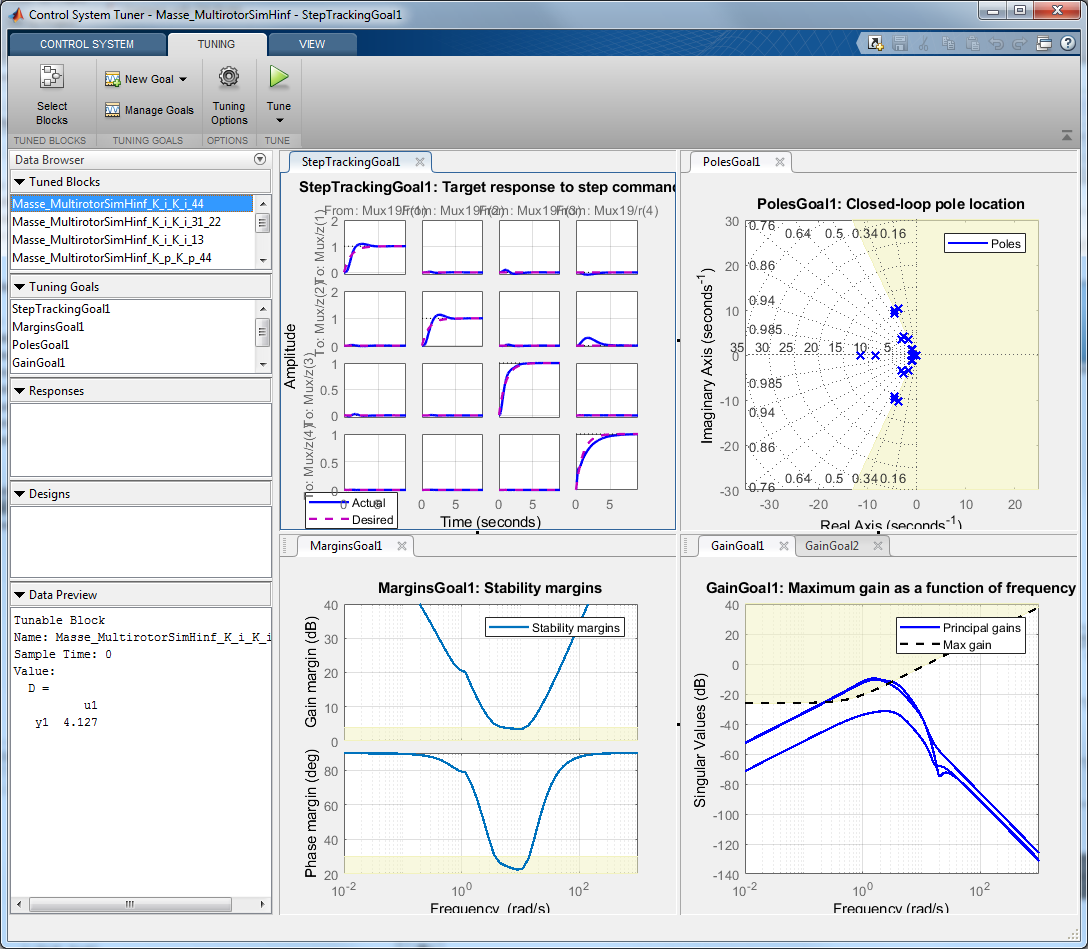
\includegraphics[width=16cm]{ctrl_systemtuner.png}%
            \caption{Simulink Control System Tuner window.}\label{fig:ctrl_systemtuner.png}
        \end{figure}

    \section{Issues with Model Implementation}\label{sec:issues}

        Several issues arose while implementing the quadcopter model presented by Mass{\'e} et al. They are listed in this section as a matter of record.

        \subsection{Khan and Nahon's Propeller Model}

            Khan and Nahon's propeller model predicts three-dimensional forces and moments generated by a propeller given the propeller parameters, its rotational speed, and an inflow wind vector. It uses a combination of blade-element and momentum theory and accounts for assymetric blade effects.

            The first step of the process is to compute the blade aerodynamic coefficients as a function of the effective angle of attack on the blade. The results presented in the paper were successfully replicated, as shown in Figure~\ref{fig:aero_coefs}.

            \begin{figure}[h!]
                \centering%
                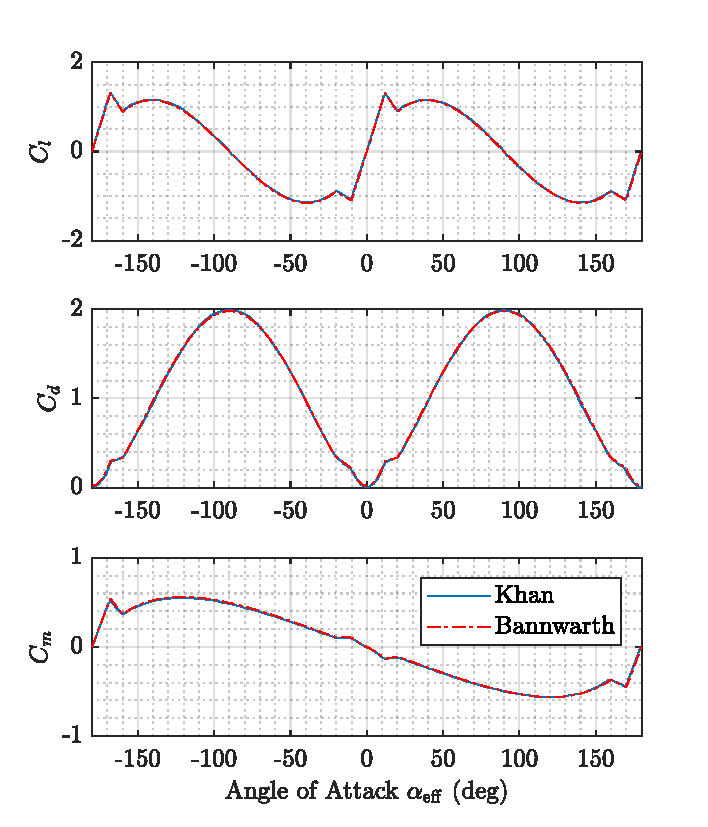
\includegraphics{aero_coefs.pdf}%
                \caption{Aerodynamic coefficients variations with angle of attack}\label{fig:aero_coefs}
            \end{figure}

            The second step consists of computing the induced axial velocity distribution on the blade as a function of the angle of the blade and distance of the element from the centre of the propeller. This was also successfully replicated.

            The third step involves the computation of the three primary forces, \(F_x\), \(F_y\), and \(F_z\), and moments, \(M_x\), \(M_y\), and \(M_z\). These equations to compute these forces and moments can be divided in two groups; those derived from Equation~\eqref{eq:dT} and those derived from Equation~\eqref{eq:dH}:
            %
            \begin{align}
                \mathrm{d} T = \frac{N}{4\pi}\rho c \int_{\psi=0}^{2\pi} V^2_R \left( C_l \cos \phi - C_d \sin \phi \right) \mathrm{d} \psi \mathrm{d} r,  \label{eq:dT} \\
                \mathrm{d} H = \frac{N}{4\pi}\rho c \int_{\psi=0}^{2\pi} V^2_R \left( C_l \sin \phi + C_d \cos \phi \right) \mathrm{d} \psi \mathrm{d} r. \label{eq:dH}
            \end{align}

            The equations for \(F_x\), \(M_y\), and \(M_z\) are derived from Equation~\eqref{eq:dT} and those for \(F_y\), \(F_z\), and \(M_x\) are derived from Equation~\eqref{eq:dH}. The former were able to be matched relatively closely, while the latter were not, as shown in~\ref{fig:aero_fm} While it is possible this is due to an implementation mistake, the equations for all forces and moments are relatively similar, and were re-derived and checked several times.

            \begin{figure}[h!]
                \centering%
                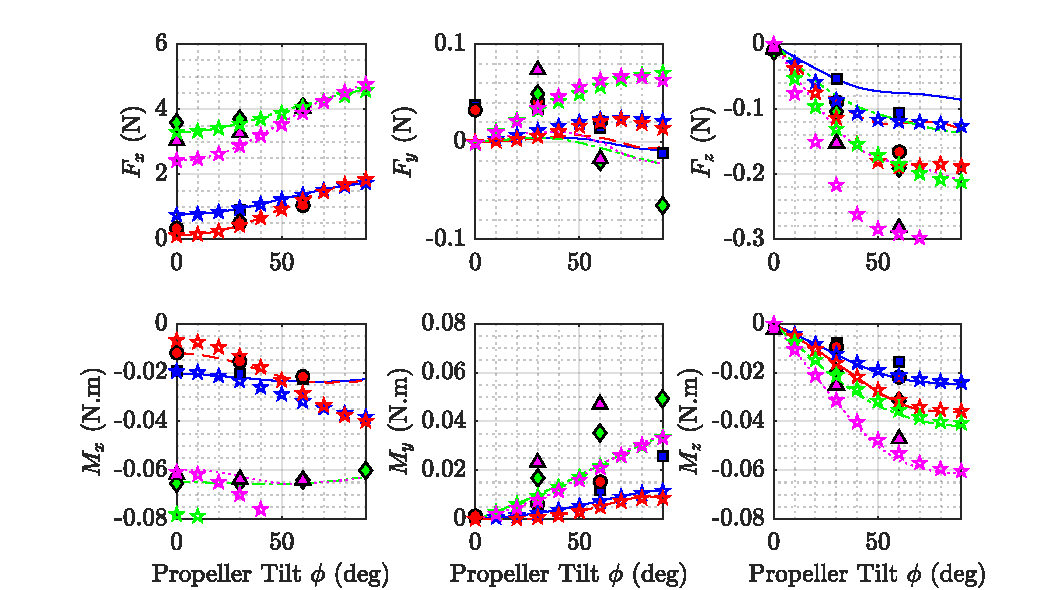
\includegraphics{aero_fm.pdf}%
                \caption{Aerodynamic forces and moments predicted by the propeller model. The solid markers and lines represent Khan et al.'s experimental and simulation results respectively, and the stars represent Bannwarth et al.'s results. These results are expressed in the UAV frame with an incident angle of the wind of \SI{90}{\degree}, which means that the \(y\) and \(z\) axes are inverted compared to the propeller frame.}\label{fig:aero_fm}
            \end{figure}

            Finally, a small mistake was found in the forces and moment equations. As an example, the equation for the axial thrust generated by the rotor is given as
            %
            \begin{align}
                T = \frac{N}{4\pi} \rho c \sum_{r=R_h}^{R_p} \sum_{\psi=0}^{2\pi} V_R^2 \left( C_l \cos \phi - C_d \sin \phi \right) \Delta \psi \Delta r.
            \end{align}

            However, the chord length \(c\) is a function of the distance of the element from the centre of the propeller, \(r\). As a consequence, it should by inside the first summation sign rather than outside, as follows:
            %
            \begin{align}
                T = \frac{N}{4\pi} \rho \sum_{r=R_h}^{R_p} c \sum_{\psi=0}^{2\pi} V_R^2 \left( C_l \cos \phi - C_d \sin \phi \right) \Delta \psi \Delta r.
            \end{align}
            
            This small correction applies to all six force and moment equations.


        \subsection{Mass{\'e} et al.'s Implementation of the Propeller Model}

            There are two main issues with Mass{\'e} et al.'s implementation of Khan and Nahon's propeller model.

            First of all, in their paper, Mass{\'e} et al.\ state that they have used generated look-up tables using Khan and Nahon's propeller model. They claim the look-up tables were generated over the following ranges of input rotor speed \(\omega_j\), axial wind speed \(u^p_a\), and in-plane wind speed \( || \begin{bmatrix} v^p_a & w^p_a \end{bmatrix} ||_2  \):

            \begin{align*}
                \omega_j &\in [0,8600] \; \text{RPM}\\
                u^p_a &\in [-12,12] \; \si{\metre\per\second}\\
                || \begin{bmatrix} v^p_a & w^p_a \end{bmatrix} ||_2 &\in [0,20] \; \si{\metre\per\second}
            \end{align*}

            The range for the angular speed and in-plane velocity is appropriate. On the other hand, Khan and Nahon's model is for forward flight, which means that it is not proven to work for negative axial wind speeds. Indeed, Khan and Nahon do not present results in the negative range in any of their papers. As a consquence, the range of axial wind speeds presented is dubious.

            The second issue lies in the computation of the forces and moments. Khan and Nahon's model computes all forces and moments generated by a propeller. However, Mass{\'e} et al.\ add the output of a standard thurst model \(\propto k_t \omega_j^2\) to that of their propeller model, which should result in a doubled amount of thrust. In addition, the forces and moments generated by the propeller model are scaled from 0 to 1 depending on the orientation of the propeller relative to the wind and the UAV. No details or rationale for this implementation are provided.

        \subsection{Controller Implementation Details}
        
            There is a number of small mistakes in the controller implementation details presented in the paper. For example, some of the gain matrices presented for the \Hinf\ controller have incorrect signs, and the given state feedback \(\mathbf{SOF}_2\) matrix has a form indicating it should be applied to the vector \(\mathbf{y}_2 = \begin{bmatrix} \dot{z} & z & p & \phi & q & \theta & r & \psi \end{bmatrix}^\top\), whereas the paper previously states that \(\mathbf{y}_2 = \begin{bmatrix} \dot{z} & p & q & r & z & \phi & \theta & \psi \end{bmatrix}^\top\).

            In addition, the paper provides a state-space model for the system and states it is used for the controller synthesis procedure. However, the state-space model does not have a disturbance input, which is necessary to synthesise a \Hinf\ controller. It is likely that Mass{\'e} et al.\ used Simulink's Control System Tuner which automatically performs a linearisation of the system dynamics, however they do not explicitely say so. This means that there is no need to replicate the state-space model provided in the paper, as numerically linearising the non-linear model using Simulink's tools is necessary anyway.

    \bibliographystyle{ieeetran}
    \bibliography{bibliography}
\end{document}